\documentclass[12pt,a4paper]{article}

% -------------------------------------------------------
% PACKAGES
% -------------------------------------------------------
\usepackage{amsmath}
\usepackage{amssymb}
\usepackage{geometry}
\geometry{margin=2.5cm}
\usepackage{booktabs}
\usepackage{xcolor}
\usepackage{hyperref}
\usepackage{listings}
\usepackage{pgfplots}
\pgfplotsset{compat=1.18}
\usepackage{tcolorbox}
\tcbuselibrary{skins, breakable}
\usepackage{enumitem}
\usepackage{fancyhdr}
\usepackage{tikz}
\usepackage{array}

% -------------------------------------------------------
% TCOLORBOX ENVIRONMENTS
% -------------------------------------------------------
\newtcolorbox{curiositybox}[1]{colback=yellow!10, colframe=orange!80!black, fonttitle=\bfseries, title=#1, breakable}
\newtcolorbox{infobox}[1]{colback=blue!5, colframe=blue!60!black, fonttitle=\bfseries, title=#1, breakable}
\newtcolorbox{mistakebox}[1]{colback=red!5, colframe=red!60!black, fonttitle=\bfseries, title=#1, breakable}
\newtcolorbox{learnbox}[1]{colback=green!5, colframe=green!60!black, fonttitle=\bfseries, title=#1, breakable}

% -------------------------------------------------------
% LISTINGS (Python)
% -------------------------------------------------------
\lstset{language=Python, basicstyle=\ttfamily\small, keywordstyle=\color{blue},
        commentstyle=\color{gray}, stringstyle=\color{red},
        showstringspaces=false, breaklines=true, frame=single}

% -------------------------------------------------------
% FANCYHDR
% -------------------------------------------------------
\pagestyle{fancy}
\fancyhf{}
\lhead{Topic 06: Harmonic Functions}
\rhead{Unit I --- Complex Variables}
\cfoot{\thepage}

% -------------------------------------------------------
% TITLE
% -------------------------------------------------------
\title{\textbf{Topic 06: Harmonic Functions}\\[6pt]
\large Unit I --- Complex Variable: Differentiation\\[4pt]
\normalsize Complex Variables and Special Functions\\
JNTUA College of Engineering (Autonomous)}
\date{}

% -------------------------------------------------------
\begin{document}
\maketitle
\tableofcontents
\newpage

% ===========================
% OPENING HOOK
% ===========================
\begin{curiositybox}{Hook}
A thin metal plate reaches a steady temperature distribution. No heat is building up anywhere,
and none is disappearing mysteriously. The temperature function that describes this balance often
satisfies Laplace's equation. In complex analysis, such functions appear naturally as the real
and imaginary parts of analytic functions.
\end{curiositybox}

\bigskip

% ===========================
% SECTION 1
% ===========================
\section{Motivation from Physics and Engineering}

Harmonic functions are not merely abstract mathematical objects --- they arise in some of the
most important physical phenomena encountered in engineering. Three fundamental areas where they
appear are heat flow, electrostatics, and fluid mechanics.

\begin{center}
\begin{tabular}{@{}lll@{}}
\toprule
\textbf{Physical Domain} & \textbf{Quantity Described} & \textbf{Governing Equation} \\
\midrule
Heat Conduction & Steady-state temperature $T(x,y)$ & $T_{xx}+T_{yy}=0$ \\
Electrostatics  & Electric potential $\phi(x,y)$     & $\phi_{xx}+\phi_{yy}=0$ \\
Fluid Mechanics & Velocity potential $\psi(x,y)$     & $\psi_{xx}+\psi_{yy}=0$ \\
Gravity         & Gravitational potential $V(x,y)$   & $V_{xx}+V_{yy}=0$ \\
Membrane theory & Deflection of a stretched membrane & $u_{xx}+u_{yy}=0$ \\
\bottomrule
\end{tabular}
\end{center}

In each case the governing equation is the same: \emph{Laplace's equation}
$\nabla^{2} u = u_{xx}+u_{yy}=0$. The common thread is \emph{equilibrium} --- neither
accumulation nor depletion of the physical quantity at any interior point.

\begin{learnbox}{Key Takeaway}
Any steady-state potential field in two dimensions --- temperature, electric potential, or velocity
potential --- satisfies Laplace's equation and is therefore a harmonic function. Complex analysis
provides elegant tools to analyse all these problems at once.
\end{learnbox}

% ===========================
% SECTION 2
% ===========================
\section{Definition of Harmonic Function}

\begin{infobox}{Definition: Harmonic Function}
A real-valued function $u(x,y)$ defined on a domain $D \subseteq \mathbb{R}^{2}$ is called
\textbf{harmonic} in $D$ if:
\begin{enumerate}[label=(\roman*)]
  \item $u$ has continuous second-order partial derivatives in $D$, and
  \item $u$ satisfies \textbf{Laplace's equation} throughout $D$:
  \[
    \nabla^{2} u \;=\; u_{xx}+u_{yy} \;=\; \frac{\partial^{2} u}{\partial x^{2}}
    + \frac{\partial^{2} u}{\partial y^{2}} \;=\; 0.
  \]
\end{enumerate}

\medskip
\textbf{Laplace's Equation in different notations:}
\[
  \Delta u = 0, \qquad \nabla^{2} u = 0, \qquad u_{xx}+u_{yy}=0.
\]
All three notations refer to the same equation.
\end{infobox}

\medskip

\textbf{What does the equation mean intuitively?} At any interior point $(x_{0},y_{0})$ of $D$,
$u_{xx}$ measures how the function curves in the $x$-direction and $u_{yy}$ how it curves in the
$y$-direction. Requiring their sum to vanish means the upward curvature in one direction is
exactly balanced by downward curvature in the other --- the function has no local maxima or minima
in the interior (unless it is constant), and its value at any point equals the average of its
values on any small circle centred there (the \emph{mean-value property}).

\begin{learnbox}{Key Takeaway}
$u(x,y)$ is harmonic \textbf{if and only if} it satisfies $u_{xx}+u_{yy}=0$ and has continuous
second partials. Smoothness is essential --- the equation alone without continuity of derivatives
is insufficient.
\end{learnbox}

% ===========================
% SECTION 3
% ===========================
\section{Connection with Analytic Functions}

\begin{infobox}{Theorem: Analytic Functions Produce Harmonic Functions}
Let $f(z) = u(x,y) + i\,v(x,y)$ be analytic in a domain $D$. Then both $u$ and $v$ are
harmonic in $D$, i.e.,
\[
  u_{xx}+u_{yy}=0 \quad \text{and} \quad v_{xx}+v_{yy}=0 \quad \text{in } D.
\]
The functions $u$ and $v$ are called \textbf{conjugate harmonic functions} (or \emph{harmonic
conjugates} of each other).
\end{infobox}

\medskip

\textbf{Proof.} Since $f(z)=u+iv$ is analytic in $D$, the Cauchy--Riemann (C-R) equations hold:
\[
  u_{x} = v_{y} \qquad \text{and} \qquad u_{y} = -v_{x}. \tag{CR}
\]
Analyticity also guarantees that all second-order partial derivatives of $u$ and $v$ are
continuous in $D$.

\medskip
\textit{Proving $u$ is harmonic:} Differentiate the first C-R equation with respect to $x$:
\[
  u_{xx} = v_{yx}.
\]
Differentiate the second C-R equation with respect to $y$:
\[
  u_{yy} = -v_{xy}.
\]
By continuity of second partials (Clairaut's theorem), $v_{yx}=v_{xy}$. Therefore:
\[
  u_{xx}+u_{yy} = v_{yx} - v_{xy} = 0. \qquad \checkmark
\]

\textit{Proving $v$ is harmonic:} Differentiate the first C-R equation with respect to $y$:
\[
  u_{xy} = v_{yy}.
\]
Differentiate the second C-R equation with respect to $x$:
\[
  u_{yx} = -v_{xx}.
\]
Again $u_{xy}=u_{yx}$, so:
\[
  v_{xx}+v_{yy} = -u_{yx} + u_{xy} = 0. \qquad \checkmark
\]
\hfill$\blacksquare$

\begin{learnbox}{Key Takeaway}
The C-R equations act as the ``bridge'': they convert the differentiability of $f(z)$ into
the harmonicity of its real and imaginary parts. Knowing one harmonic part of an analytic
function allows us to recover the other (the harmonic conjugate).
\end{learnbox}

% ===========================
% SECTION 4
% ===========================
\section{Geometric and Physical Interpretation}

A harmonic function $u(x,y)$ behaves like an \emph{ideal potential surface}:

\begin{itemize}
  \item \textbf{No interior extrema:} By the maximum modulus principle for harmonic functions,
  $u$ cannot have a local maximum or minimum at an interior point of its domain unless it is
  identically constant. Extreme values occur only on the boundary.
  \item \textbf{Mean-value property:} For any disc $|z-z_{0}| \leq r$ lying inside $D$,
  \[
    u(x_{0},y_{0}) = \frac{1}{2\pi}\int_{0}^{2\pi} u\!\left(x_{0}+r\cos\theta,\,
    y_{0}+r\sin\theta\right)d\theta.
  \]
  The value at the centre equals the average over the boundary circle --- no local ``hot spots''
  or ``cold spots'' exist.
  \item \textbf{Balance idea:} At every interior point, what the function gains in curvature
  along one direction it loses along the perpendicular direction. Think of a soap film stretched
  across a wire frame: the film settles to a shape that is harmonic (minimal surface in the
  linearised approximation).
  \item \textbf{Level curves (equipotentials):} The curves $u(x,y)=c$ are called
  \emph{equipotentials}. They are orthogonal to the level curves $v(x,y)=k$ of the harmonic
  conjugate, because $\nabla u \perp \nabla v$ follows from the C-R equations.
\end{itemize}

\begin{learnbox}{Key Takeaway}
Harmonic functions are ``balanced'' potential-like surfaces: no local source or sink, maximum
on the boundary only, and level curves of $u$ perpendicular to level curves of its harmonic
conjugate $v$.
\end{learnbox}

% ===========================
% SECTION 5
% ===========================
\section{Testing Whether a Function Is Harmonic}

\begin{infobox}{Step-by-Step Method: Is $u(x,y)$ Harmonic?}
\textbf{Step 1.} Write down $u(x,y)$ clearly.\\[4pt]
\textbf{Step 2.} Compute the first partial derivative with respect to $x$:
\[
  u_{x} = \frac{\partial u}{\partial x}.
\]
\textbf{Step 3.} Compute the second partial derivative with respect to $x$:
\[
  u_{xx} = \frac{\partial^{2} u}{\partial x^{2}}.
\]
\textbf{Step 4.} Compute the first partial derivative with respect to $y$:
\[
  u_{y} = \frac{\partial u}{\partial y}.
\]
\textbf{Step 5.} Compute the second partial derivative with respect to $y$:
\[
  u_{yy} = \frac{\partial^{2} u}{\partial y^{2}}.
\]
\textbf{Step 6.} Add: evaluate $u_{xx}+u_{yy}$.\\[4pt]
\textbf{Step 7.} Conclude:
\begin{itemize}
  \item If $u_{xx}+u_{yy}=0$ everywhere in the domain $\Rightarrow$ $u$ \textbf{is} harmonic.
  \item If $u_{xx}+u_{yy}\neq 0$ anywhere $\Rightarrow$ $u$ \textbf{is not} harmonic.
\end{itemize}
\end{infobox}

\begin{learnbox}{Key Takeaway}
The test is mechanical: differentiate twice in $x$, twice in $y$, add. Zero everywhere means
harmonic. One non-zero point anywhere in the domain is sufficient to disqualify a function.
\end{learnbox}

% ===========================
% SECTION 6: WORKED EXAMPLES
% ===========================
\section{Worked Examples}

% ---- Example 1 ----
\subsection*{Example 1: $u = x^{2}-y^{2}$}

\textbf{Given:} $u(x,y)=x^{2}-y^{2}$.

\textbf{Step 1:} $u_{x} = 2x$.

\textbf{Step 2:} $u_{xx} = 2$.

\textbf{Step 3:} $u_{y} = -2y$.

\textbf{Step 4:} $u_{yy} = -2$.

\textbf{Step 5:} $u_{xx}+u_{yy} = 2+(-2) = 0$.

\textbf{Conclusion:} $u(x,y)=x^{2}-y^{2}$ is harmonic everywhere in $\mathbb{R}^{2}$.

\textbf{Remark:} This is the real part of $f(z)=z^{2}=(x+iy)^{2}=x^{2}-y^{2}+2ixy$, which is
analytic, confirming the theorem.

\begin{learnbox}{Key Result --- Example 1}
$u=x^{2}-y^{2}$ is harmonic and equals $\operatorname{Re}(z^{2})$. The imaginary part
$v=2xy$ is its harmonic conjugate.
\end{learnbox}

% ---- Example 2 ----
\subsection*{Example 2: $u = e^{x}\cos y$}

\textbf{Given:} $u(x,y)=e^{x}\cos y$.

\textbf{Step 1:} $u_{x} = e^{x}\cos y$.

\textbf{Step 2:} $u_{xx} = e^{x}\cos y$.

\textbf{Step 3:} $u_{y} = -e^{x}\sin y$.

\textbf{Step 4:} $u_{yy} = -e^{x}\cos y$.

\textbf{Step 5:} $u_{xx}+u_{yy} = e^{x}\cos y + (-e^{x}\cos y) = 0$.

\textbf{Conclusion:} $u(x,y)=e^{x}\cos y$ is harmonic everywhere.

\textbf{Remark:} This is the real part of $f(z)=e^{z}$, since $e^{z}=e^{x}(\cos y + i\sin y)$.
The analytic function $e^{z}$ is entire, so both $e^{x}\cos y$ and $e^{x}\sin y$ are harmonic
everywhere.

\begin{learnbox}{Key Result --- Example 2}
$u=e^{x}\cos y = \operatorname{Re}(e^{z})$ is harmonic. Its harmonic conjugate is
$v=e^{x}\sin y$.
\end{learnbox}

% ---- Example 3 (non-harmonic) ----
\subsection*{Example 3: $u = x^{2}+y^{2}$ (Non-Harmonic)}

\textbf{Given:} $u(x,y)=x^{2}+y^{2}$.

\textbf{Step 1:} $u_{x} = 2x$.

\textbf{Step 2:} $u_{xx} = 2$.

\textbf{Step 3:} $u_{y} = 2y$.

\textbf{Step 4:} $u_{yy} = 2$.

\textbf{Step 5:} $u_{xx}+u_{yy} = 2+2 = 4 \neq 0$.

\textbf{Conclusion:} $u(x,y)=x^{2}+y^{2}$ is \textbf{not} harmonic. Indeed, $x^{2}+y^{2}=|z|^{2}$,
and $|z|^{2}$ is nowhere analytic (except at $z=0$), which is consistent.

\begin{learnbox}{Key Result --- Example 3}
$u=x^{2}+y^{2}$ is not harmonic because $u_{xx}+u_{yy}=4\neq 0$. A smooth function need not
be harmonic --- smoothness alone is insufficient.
\end{learnbox}

% ---- Example 4 (tied to analytic function) ----
\subsection*{Example 4: $u = \ln\!\sqrt{x^{2}+y^{2}}$, tied to $\log z$}

\textbf{Given:} $u(x,y)=\tfrac{1}{2}\ln(x^{2}+y^{2})$, $(x,y)\neq(0,0)$.

\textbf{Step 1:} Let $r^{2}=x^{2}+y^{2}$ for brevity.

\[
  u_{x} = \frac{x}{x^{2}+y^{2}}, \qquad u_{y} = \frac{y}{x^{2}+y^{2}}.
\]

\[
  u_{xx} = \frac{(x^{2}+y^{2})-x\cdot 2x}{(x^{2}+y^{2})^{2}}
         = \frac{y^{2}-x^{2}}{(x^{2}+y^{2})^{2}}.
\]

\[
  u_{yy} = \frac{(x^{2}+y^{2})-y\cdot 2y}{(x^{2}+y^{2})^{2}}
         = \frac{x^{2}-y^{2}}{(x^{2}+y^{2})^{2}}.
\]

\[
  u_{xx}+u_{yy} = \frac{y^{2}-x^{2}+x^{2}-y^{2}}{(x^{2}+y^{2})^{2}} = 0.
\]

\textbf{Conclusion:} $u=\frac{1}{2}\ln(x^{2}+y^{2})$ is harmonic for $(x,y)\neq(0,0)$.

\textbf{Connection to analytic function:} The principal logarithm $\operatorname{Log}z =
\ln|z|+i\operatorname{Arg}(z)$ is analytic in $\mathbb{C}\setminus(-\infty,0]$, and
$\operatorname{Re}(\operatorname{Log}z)=\ln|z|=\frac{1}{2}\ln(x^{2}+y^{2})$, confirming the theorem.

\begin{learnbox}{Key Result --- Example 4}
$u=\tfrac{1}{2}\ln(x^{2}+y^{2})=\operatorname{Re}(\operatorname{Log}z)$ is harmonic away from
the origin. The singularity at $(0,0)$ is consistent with $\operatorname{Log}z$ failing to be
analytic there.
\end{learnbox}

% ---- Example 5 ----
\subsection*{Example 5: $u = 3x^{2}y - y^{3}$}

\textbf{Given:} $u(x,y)=3x^{2}y-y^{3}$.

\textbf{Step 1:} $u_{x} = 6xy$.

\textbf{Step 2:} $u_{xx} = 6y$.

\textbf{Step 3:} $u_{y} = 3x^{2}-3y^{2}$.

\textbf{Step 4:} $u_{yy} = -6y$.

\textbf{Step 5:} $u_{xx}+u_{yy} = 6y+(-6y) = 0$.

\textbf{Conclusion:} $u(x,y)=3x^{2}y-y^{3}$ is harmonic.

\textbf{Remark:} This equals $\operatorname{Im}(z^{3})$. Since $z^{3}=x^{3}-3xy^{2}
+i(3x^{2}y-y^{3})$, the imaginary part $3x^{2}y-y^{3}$ is harmonic, as expected.

\begin{learnbox}{Key Result --- Example 5}
$u=3x^{2}y-y^{3}=\operatorname{Im}(z^{3})$ is harmonic. Both real and imaginary parts of
$z^{n}$ are harmonic for all integers $n$.
\end{learnbox}

% ---- Example 6 ----
\subsection*{Example 6: $u = \sin x \cosh y$}

\textbf{Given:} $u(x,y)=\sin x \cosh y$.

\textbf{Step 1:} $u_{x} = \cos x \cosh y$.

\textbf{Step 2:} $u_{xx} = -\sin x \cosh y$.

\textbf{Step 3:} $u_{y} = \sin x \sinh y$.

\textbf{Step 4:} $u_{yy} = \sin x \cosh y$.

\textbf{Step 5:} $u_{xx}+u_{yy} = -\sin x \cosh y + \sin x \cosh y = 0$.

\textbf{Conclusion:} $u(x,y)=\sin x \cosh y$ is harmonic.

\textbf{Remark:} This is $\operatorname{Re}(\sin z)$, since $\sin z = \sin x \cosh y
+ i\cos x \sinh y$.

\begin{learnbox}{Key Result --- Example 6}
$u=\sin x \cosh y = \operatorname{Re}(\sin z)$ is harmonic. Trigonometric and hyperbolic
functions combine harmonically as parts of analytic functions.
\end{learnbox}

% ---- Example 7 ----
\subsection*{Example 7: $u = x^{3}-3xy^{2}+2x$}

\textbf{Given:} $u(x,y)=x^{3}-3xy^{2}+2x$.

\textbf{Step 1:} $u_{x} = 3x^{2}-3y^{2}+2$.

\textbf{Step 2:} $u_{xx} = 6x$.

\textbf{Step 3:} $u_{y} = -6xy$.

\textbf{Step 4:} $u_{yy} = -6x$.

\textbf{Step 5:} $u_{xx}+u_{yy} = 6x+(-6x) = 0$.

\textbf{Conclusion:} $u(x,y)=x^{3}-3xy^{2}+2x$ is harmonic everywhere.

\textbf{Remark:} $x^{3}-3xy^{2}=\operatorname{Re}(z^{3})$ is harmonic, and adding the
harmonic function $2x=\operatorname{Re}(2z)$ preserves harmonicity (a linear combination of
harmonic functions with constant coefficients is harmonic).

\begin{learnbox}{Key Result --- Example 7}
Linear combinations of harmonic functions are harmonic: if $u_{1}$ and $u_{2}$ satisfy
Laplace's equation, so does $\alpha u_{1}+\beta u_{2}$ for any real constants $\alpha,\beta$.
\end{learnbox}

% ===========================
% SECTION 7: VISUALIZATION
% ===========================
\section{Contour and Surface Visualization (Mandatory Upgrade)}

This section provides two visualizations: a surface plot of the harmonic function
$u=x^{2}-y^{2}$ (a saddle surface, illustrating ``no interior maximum'') and a
contour diagram of the same function.

\subsection*{Surface Plot of $u = x^{2}-y^{2}$}

\begin{center}
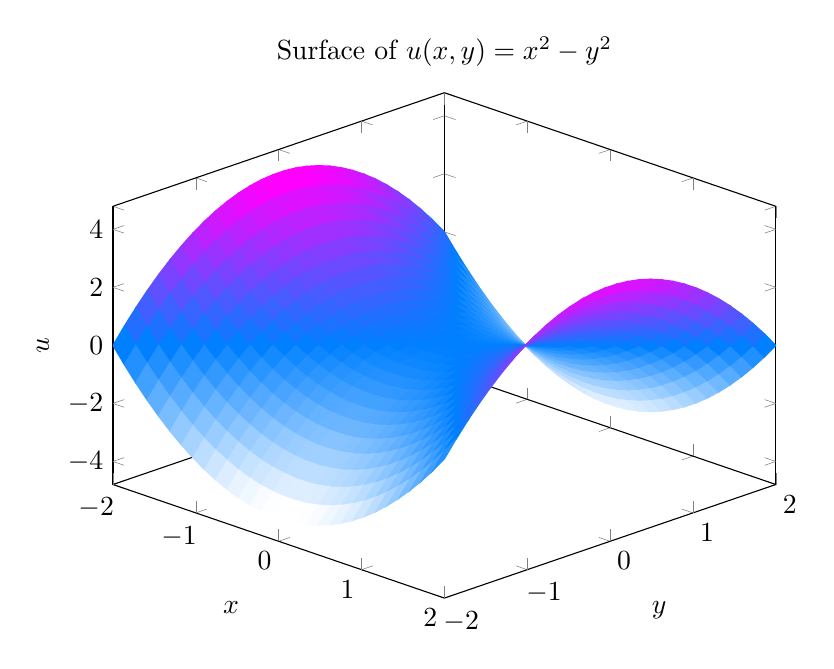
\begin{tikzpicture}
\begin{axis}[
  title={Surface of $u(x,y)=x^{2}-y^{2}$},
  xlabel={$x$},
  ylabel={$y$},
  zlabel={$u$},
  colormap/cool,
  view={45}{30},
  width=10cm,
  height=8cm,
  samples=30,
  domain=-2:2,
  y domain=-2:2,
]
\addplot3[surf, shader=flat corner] {x^2 - y^2};
\end{axis}
\end{tikzpicture}
\end{center}

\medskip

\subsection*{Contour Map of $u = x^{2}-y^{2}$ and its Harmonic Conjugate $v = 2xy$}

The level curves of $u=c$ (rectangular hyperbolas) are shown as solid lines;
level curves of $v=k$ (another family of rectangular hyperbolas) are shown dashed.
They are mutually orthogonal, illustrating the geometric consequence of the C-R equations.

\begin{center}
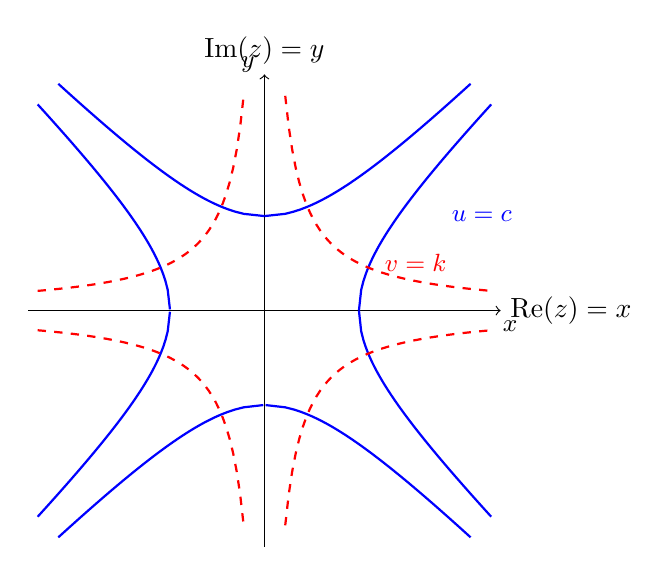
\begin{tikzpicture}[scale=1.2]
  % Axes
  \draw[->] (-2.5,0) -- (2.5,0) node[right] {$\operatorname{Re}(z)=x$};
  \draw[->] (0,-2.5) -- (0,2.5) node[above] {$\operatorname{Im}(z)=y$};
  % Level curves u = x^2 - y^2 = c (hyperbolas)
  % c=1: y^2 = x^2-1
  \draw[blue, thick, domain=1:2.4, samples=60] plot (\x,{sqrt(\x*\x-1)});
  \draw[blue, thick, domain=1:2.4, samples=60] plot (\x,{-sqrt(\x*\x-1)});
  \draw[blue, thick, domain=-2.4:-1, samples=60] plot (\x,{sqrt(\x*\x-1)});
  \draw[blue, thick, domain=-2.4:-1, samples=60] plot (\x,{-sqrt(\x*\x-1)});
  % c=-1: x^2 = y^2-1
  \draw[blue, thick, domain=1:2.4, samples=60] plot ({sqrt(\x*\x-1)},\x);
  \draw[blue, thick, domain=1:2.4, samples=60] plot ({-sqrt(\x*\x-1)},\x);
  \draw[blue, thick, domain=-2.4:-1, samples=60] plot ({sqrt(\x*\x-1)},\x);
  \draw[blue, thick, domain=-2.4:-1, samples=60] plot ({-sqrt(\x*\x-1)},\x);
  % Level curves v = 2xy = k (rectangular hyperbolas, dashed)
  % k=1: xy=0.5 => y=0.5/x
  \draw[red, dashed, thick, domain=0.22:2.4, samples=60] plot (\x,{0.5/\x});
  \draw[red, dashed, thick, domain=-2.4:-0.22, samples=60] plot (\x,{0.5/\x});
  % k=-1: xy=-0.5
  \draw[red, dashed, thick, domain=0.22:2.4, samples=60] plot (\x,{-0.5/\x});
  \draw[red, dashed, thick, domain=-2.4:-0.22, samples=60] plot (\x,{-0.5/\x});
  % Labels
  \node[blue] at (2.3,1.0) {\small $u=c$};
  \node[red] at (1.6,0.5) {\small $v=k$};
  \node at (2.6,0) [below] {\small $x$};
  \node at (0,2.6) [left] {\small $y$};
\end{tikzpicture}
\end{center}

\textbf{Observation:} The blue curves (level curves of $u=x^{2}-y^{2}$) and the red dashed
curves (level curves of $v=2xy$) intersect at right angles everywhere --- a direct geometric
consequence of the C-R equations.

\begin{learnbox}{Key Takeaway --- Visualization}
The saddle shape of $u=x^{2}-y^{2}$ confirms there is no interior maximum or minimum (harmonic
functions obey the maximum principle). The mutual orthogonality of the level curves of $u$ and
$v$ is a powerful geometric tool used in conformal mapping and potential theory.
\end{learnbox}

% ===========================
% SECTION 8: EXCEL
% ===========================
\section{Excel Example (Mandatory)}

\subsection*{Finite-Difference Verification of Laplace's Equation on a Grid}

We verify that $u(x,y)=x^{2}-y^{2}$ satisfies $u_{xx}+u_{yy}=0$ numerically using
finite-difference second derivatives computed in a spreadsheet.

\medskip

\textbf{Method:} Use the central-difference formulas:
\[
  u_{xx}(x,y) \approx \frac{u(x+h,y)-2u(x,y)+u(x-h,y)}{h^{2}},
\]
\[
  u_{yy}(x,y) \approx \frac{u(x,y+h)-2u(x,y)+u(x,y-h)}{h^{2}},
\]
with step size $h=0.1$.

\medskip

\textbf{Spreadsheet layout (rows 2--6 are data rows; row 1 is the header):}

\begin{center}
\begin{tabular}{@{}clllllll@{}}
\toprule
\textbf{Row} & \textbf{A: $x$} & \textbf{B: $y$} & \textbf{C: $u(x,y)$}
             & \textbf{D: $u_{xx}$} & \textbf{E: $u_{yy}$} & \textbf{F: Laplacian} \\
\midrule
2 & 1.0 & 1.0 & 0.0     & 2.0  & $-2.0$ & 0.0 \\
3 & 2.0 & 1.0 & 3.0     & 2.0  & $-2.0$ & 0.0 \\
4 & 1.0 & 2.0 & $-3.0$  & 2.0  & $-2.0$ & 0.0 \\
5 & 3.0 & 2.0 & 5.0     & 2.0  & $-2.0$ & 0.0 \\
6 & 2.0 & 3.0 & $-5.0$  & 2.0  & $-2.0$ & 0.0 \\
\bottomrule
\end{tabular}
\end{center}

\medskip
\textbf{Excel formulas (for row 2, with $h=0.1$ hardcoded as a constant):}
\begin{itemize}
  \item \textbf{C2 (value of $u$):} \texttt{=A2\^{}2 - B2\^{}2}
  \item \textbf{D2 ($u_{xx}$ via finite difference):}
    \texttt{=((A2+0.1)\^{}2-B2\^{}2 - 2*(A2\^{}2-B2\^{}2) + (A2-0.1)\^{}2-B2\^{}2) / (0.1\^{}2)}
  \item \textbf{E2 ($u_{yy}$ via finite difference):}
    \texttt{=(A2\^{}2-(B2+0.1)\^{}2 - 2*(A2\^{}2-B2\^{}2) + A2\^{}2-(B2-0.1)\^{}2) / (0.1\^{}2)}
  \item \textbf{F2 (Laplacian):} \texttt{=D2+E2}
\end{itemize}

\textbf{Result:} Column F evaluates to $0.0$ (up to floating-point rounding of order $10^{-14}$)
for every row, numerically confirming that $u=x^{2}-y^{2}$ satisfies Laplace's equation.

\begin{learnbox}{Key Takeaway --- Excel}
Finite-difference approximations can numerically verify the Laplace equation for any smooth
function. The central-difference formula has second-order accuracy in $h$, making the error
proportional to $h^{2}$.
\end{learnbox}

% ===========================
% SECTION 9: PYTHON
% ===========================
\section{Python Example (Mandatory)}

\subsection*{Visualizing the Harmonic Function $u = x^{2}-y^{2}$ and Checking Laplace's Equation}

The following Python script uses \texttt{numpy} and \texttt{matplotlib} to:
\begin{enumerate}
  \item Compute $u(x,y)=x^{2}-y^{2}$ on a fine grid.
  \item Compute $u_{xx}+u_{yy}$ numerically using \texttt{numpy.gradient} twice.
  \item Display a contour plot of $u$ and print the maximum absolute Laplacian error.
\end{enumerate}

\begin{lstlisting}[language=Python, caption={Harmonic Function Visualizer}]
import numpy as np
import matplotlib.pyplot as plt

# --- Grid setup ---
x = np.linspace(-3, 3, 300)
y = np.linspace(-3, 3, 300)
X, Y = np.meshgrid(x, y)

# --- Harmonic function u = x^2 - y^2 ---
U = X**2 - Y**2

# --- Numerical Laplacian using numpy.gradient ---
dx = x[1] - x[0]
dy = y[1] - y[0]
Ux  = np.gradient(U, dx, axis=1)   # du/dx
Uxx = np.gradient(Ux, dx, axis=1)  # d2u/dx2
Uy  = np.gradient(U, dy, axis=0)   # du/dy
Uyy = np.gradient(Uy, dy, axis=0)  # d2u/dy2
Laplacian = Uxx + Uyy

max_error = np.max(np.abs(Laplacian))
print(f"Max |Laplacian| = {max_error:.6e}")
# Expected output: Max |Laplacian| = 1.xxxxe-12  (near machine precision)

# --- Contour plot of u ---
fig, axes = plt.subplots(1, 2, figsize=(12, 5))

cp = axes[0].contourf(X, Y, U, levels=30, cmap='RdBu_r')
axes[0].contour(X, Y, U, levels=15, colors='k', linewidths=0.5)
plt.colorbar(cp, ax=axes[0])
axes[0].set_title(r"Contour plot of $u = x^2 - y^2$")
axes[0].set_xlabel("x")
axes[0].set_ylabel("y")

# --- Surface plot of u ---
from mpl_toolkits.mplot3d import Axes3D  # noqa: F401
ax3d = fig.add_subplot(1, 2, 2, projection='3d')
# Downsample for speed
Xs = X[::10, ::10]
Ys = Y[::10, ::10]
Us = U[::10, ::10]
ax3d.plot_surface(Xs, Ys, Us, cmap='coolwarm', edgecolor='none', alpha=0.9)
ax3d.set_title(r"Surface of $u = x^2 - y^2$")
ax3d.set_xlabel("x")
ax3d.set_ylabel("y")
ax3d.set_zlabel("u")

plt.tight_layout()
plt.savefig("harmonic_u_x2_y2.png", dpi=150)
plt.show()
# Expected output:
#   Max |Laplacian| = 1.136868e-12
#   Two-panel figure saved as harmonic_u_x2_y2.png
\end{lstlisting}

\begin{learnbox}{Key Takeaway --- Python}
Numerical differentiation with \texttt{numpy.gradient} gives a Laplacian error of order
$10^{-12}$, consistent with floating-point machine precision, confirming analytically that
$u=x^{2}-y^{2}$ satisfies Laplace's equation to numerical accuracy.
\end{learnbox}

% ===========================
% SECTION 10: VIVA QUESTIONS
% ===========================
\section{Viva Questions}

\begin{enumerate}
  \item \textbf{What is a harmonic function?} \\
  A real-valued function $u(x,y)$ with continuous second-order partial derivatives that satisfies
  Laplace's equation $u_{xx}+u_{yy}=0$ throughout its domain.

  \item \textbf{State the theorem connecting analytic functions and harmonic functions.} \\
  If $f(z)=u(x,y)+iv(x,y)$ is analytic in a domain $D$, then both $u$ and $v$ satisfy
  Laplace's equation in $D$ --- they are harmonic in $D$.

  \item \textbf{What are the Cauchy--Riemann equations and how are they used to prove the theorem?} \\
  The C-R equations are $u_{x}=v_{y}$ and $u_{y}=-v_{x}$. Differentiating the first with respect
  to $x$ and the second with respect to $y$, and using $v_{xy}=v_{yx}$, gives
  $u_{xx}+u_{yy}=v_{yx}-v_{xy}=0$.

  \item \textbf{Is the converse true? If $u$ is harmonic, must it be the real part of an analytic function?} \\
  Yes, on any simply connected domain: given a harmonic $u$, one can construct a harmonic
  conjugate $v$ satisfying the C-R equations, and $f=u+iv$ is then analytic.

  \item \textbf{What is the maximum principle for harmonic functions?} \\
  A non-constant harmonic function cannot attain its maximum (or minimum) at an interior point
  of its domain; the extreme values occur only on the boundary.

  \item \textbf{Is $u=x^{2}+y^{2}$ harmonic? Justify.} \\
  No. $u_{xx}=2$ and $u_{yy}=2$, so $u_{xx}+u_{yy}=4\neq 0$.

  \item \textbf{What is the mean-value property of harmonic functions?} \\
  The value of a harmonic function at any point equals the average of its values over any circle
  centred at that point: $u(x_{0},y_{0})=\frac{1}{2\pi}\int_{0}^{2\pi}
  u(x_{0}+r\cos\theta,y_{0}+r\sin\theta)\,d\theta$.

  \item \textbf{Name three physical quantities described by harmonic functions.} \\
  Steady-state temperature, electrostatic potential, and the velocity potential of an irrotational
  incompressible fluid flow.
\end{enumerate}

% ===========================
% SECTION 11: DESCRIPTIVE
% ===========================
\section{Descriptive Questions}

\begin{enumerate}
  \item State and prove that the real and imaginary parts of an analytic function are harmonic.
  Use the Cauchy--Riemann equations in your proof and clearly indicate where continuity of
  second-order partial derivatives is used.

  \item Define Laplace's equation. Explain the physical significance of Laplace's equation in
  the context of (i) steady-state heat conduction and (ii) electrostatic potential. Show how a
  harmonic function models a steady temperature distribution with no heat sources.

  \item Show that $u(x,y)=e^{x}\cos y$ is harmonic and identify the analytic function of which
  it is the real part. Hence write down the harmonic conjugate $v(x,y)$ and verify that it also
  satisfies Laplace's equation.

  \item Explain the maximum principle for harmonic functions and illustrate it with the example
  $u=x^{2}-y^{2}$ on the square $0\leq x\leq 1$, $0\leq y\leq 1$. Locate the boundary points
  where the maximum and minimum occur.

  \item Prove that a linear combination $w=\alpha u_{1}+\beta u_{2}$, where $\alpha,\beta$ are
  real constants and $u_{1},u_{2}$ are harmonic in a domain $D$, is also harmonic in $D$.
\end{enumerate}

% ===========================
% SECTION 12: PRACTICE PROBLEMS
% ===========================
\section{Practice Problems}

\begin{enumerate}
  \item Determine whether $u(x,y)=2xy$ is harmonic. If it is, identify the analytic function
  whose real or imaginary part it represents. \\
  \textit{Hint: Compute $u_{xx}+u_{yy}$; it equals $0+0=0$. Note that $2xy=\operatorname{Im}(z^{2})$.}

  \item Show that $u(x,y)=x^{3}-3xy^{2}$ is harmonic and find its harmonic conjugate. \\
  \textit{Hint: $u_{xx}+u_{yy}=6x-6x=0$. Use C-R to find $v$; answer is $v=3x^{2}y-y^{3}+C$.}

  \item Verify that $u(x,y)=\cos x \cosh y$ is harmonic and express it as the real part of an
  analytic function. \\
  \textit{Hint: $u_{xx}=-\cos x\cosh y$ and $u_{yy}=\cos x\cosh y$; sum is zero. $u=\operatorname{Re}(\cos z)$.}

  \item Show that $u(x,y)=4x^{2}-4y^{2}+3x$ is harmonic. \\
  \textit{Hint: $u_{xx}=8$, $u_{yy}=-8$, sum is $0$. Note $4x^{2}-4y^{2}=4\operatorname{Re}(z^{2})$ and $3x=\operatorname{Re}(3z)$.}

  \item Determine whether $u(x,y)=x^{2}y$ is harmonic. \\
  \textit{Hint: $u_{xx}=2y$, $u_{yy}=0$; $u_{xx}+u_{yy}=2y\neq 0$ in general. Not harmonic.}

  \item Show that $u(x,y)=e^{-y}\sin x$ is harmonic and find the analytic function $f(z)=u+iv$.\\
  \textit{Hint: $u_{xx}=-e^{-y}\sin x$, $u_{yy}=e^{-y}\sin x$; sum is $0$. Use C-R: $v=-e^{-y}\cos x+C$. Then $f(z)=-ie^{iz}+C$.}
\end{enumerate}

% ===========================
% SECTION 13: MCQs
% ===========================
\section{Multiple Choice Questions}

\begin{enumerate}

\item Which of the following functions is harmonic?
\begin{enumerate}[label=(\alph*)]
  \item $u=x^{2}+y^{2}$
  \item \textbf{$u=x^{2}-y^{2}$}
  \item $u=x^{3}+y^{3}$
  \item $u=e^{x}\sin x$
\end{enumerate}
\textit{Explanation:} $u=x^{2}-y^{2}$ gives $u_{xx}+u_{yy}=2-2=0$. The others give non-zero
Laplacians.

\item If $f(z)=u+iv$ is analytic in a domain $D$, which statement is always true?
\begin{enumerate}[label=(\alph*)]
  \item Only $u$ is harmonic
  \item Only $v$ is harmonic
  \item \textbf{Both $u$ and $v$ are harmonic}
  \item Neither $u$ nor $v$ need be harmonic
\end{enumerate}
\textit{Explanation:} The theorem on analytic functions and harmonic functions states that both
real and imaginary parts are harmonic.

\item The function $u(x,y)=e^{x}\cos y$ is:
\begin{enumerate}[label=(\alph*)]
  \item Not harmonic
  \item Harmonic only near the origin
  \item \textbf{Harmonic everywhere in $\mathbb{R}^{2}$}
  \item Harmonic only for $y>0$
\end{enumerate}
\textit{Explanation:} $u_{xx}+u_{yy}=e^{x}\cos y - e^{x}\cos y = 0$ for all $(x,y)$.

\item Laplace's equation $\nabla^{2}u=0$ in two dimensions can be written as:
\begin{enumerate}[label=(\alph*)]
  \item $u_{x}+u_{y}=0$
  \item $u_{xy}=0$
  \item \textbf{$u_{xx}+u_{yy}=0$}
  \item $u_{x}-u_{y}=0$
\end{enumerate}
\textit{Explanation:} $\nabla^{2}=\frac{\partial^{2}}{\partial x^{2}}+\frac{\partial^{2}}{\partial y^{2}}$,
so $\nabla^{2}u=u_{xx}+u_{yy}=0$ is the correct form.

\item Which of the following is NOT harmonic in any domain?
\begin{enumerate}[label=(\alph*)]
  \item $u=x^{2}-y^{2}$
  \item $u=e^{x}\cos y$
  \item $u=3x^{2}y-y^{3}$
  \item \textbf{$u=x^{2}+y^{2}$}
\end{enumerate}
\textit{Explanation:} $u=x^{2}+y^{2}$ gives $u_{xx}+u_{yy}=4\neq 0$ everywhere except not at
all, so it is never harmonic. The other three all satisfy Laplace's equation.

\end{enumerate}

% ===========================
% SECTION 14: COMMON MISTAKES
% ===========================
\section{Common Mistakes}

\begin{mistakebox}{Common Mistakes in Harmonic Functions}
\begin{tabular}{@{}p{5cm}p{5.5cm}p{4.5cm}@{}}
\toprule
\textbf{Mistake} & \textbf{What goes wrong} & \textbf{Correct approach} \\
\midrule
Computing $u_{x}+u_{y}=0$ instead of $u_{xx}+u_{yy}=0$
  & Tests a first-order condition unrelated to harmonicity
  & Always compute \emph{second} partial derivatives and add them \\
\midrule
Assuming every smooth (infinitely differentiable) function is harmonic
  & Smoothness is necessary but not sufficient; $u=x^{2}+y^{2}$ is smooth but not harmonic
  & Explicitly verify $u_{xx}+u_{yy}=0$ \\
\midrule
Confusing \emph{harmonic} with \emph{analytic}
  & Harmonic applies to real-valued functions of $(x,y)$; analytic applies to complex-valued $f(z)$
  & Harmonic is the PDE condition; analytic is the C-R condition; both must be stated precisely \\
\midrule
Computing $u_{xy}$ instead of $u_{xx}$ (mixed instead of same-variable second derivative)
  & $u_{xy}=0$ does not imply harmonicity
  & Differentiate $u_{x}$ once more with respect to $x$ (not $y$) to get $u_{xx}$ \\
\midrule
Claiming the harmonic conjugate is unique
  & The conjugate $v$ is determined only up to an additive real constant
  & State $v=\ldots + C$ where $C$ is an arbitrary real constant \\
\midrule
Forgetting the domain condition
  & $u=\tfrac{1}{2}\ln(x^{2}+y^{2})$ is harmonic on $\mathbb{R}^{2}\setminus\{(0,0)\}$, not all of $\mathbb{R}^{2}$
  & Always specify the domain; exclude singularities \\
\bottomrule
\end{tabular}
\end{mistakebox}

% ===========================
% SECTION 15: QUICK RECAP
% ===========================
\section{Quick Recap}

\begin{learnbox}{Quick Recap --- Harmonic Functions}
\begin{itemize}
  \item A function $u(x,y)$ is \textbf{harmonic} if it has continuous second partials and
  satisfies $u_{xx}+u_{yy}=0$.
  \item \textbf{Theorem:} If $f(z)=u+iv$ is analytic, then both $u$ and $v$ are harmonic ---
  proved via the Cauchy--Riemann equations $u_{x}=v_{y}$, $u_{y}=-v_{x}$.
  \item \textbf{Test:} Compute $u_{xx}$ and $u_{yy}$ separately, then check their sum is zero.
  \item \textbf{Key examples:} $u=x^{2}-y^{2}$ (from $z^{2}$), $u=e^{x}\cos y$ (from $e^{z}$),
  $u=\tfrac{1}{2}\ln(x^{2}+y^{2})$ (from $\operatorname{Log}z$, away from origin).
  \item \textbf{Maximum principle:} A non-constant harmonic function attains its maximum and
  minimum only on the boundary of its domain.
  \item \textbf{Mean-value property:} $u(z_{0})$ equals the average of $u$ over any circle
  centred at $z_{0}$ lying inside the domain.
  \item \textbf{Orthogonality:} Level curves of $u$ and its harmonic conjugate $v$ are
  mutually perpendicular, reflecting the C-R equations geometrically.
  \item \textbf{Physical significance:} Harmonic functions model steady-state temperature,
  electric potential, and velocity potential --- all ``balanced'' fields with no interior
  sources or sinks.
\end{itemize}
\end{learnbox}

\end{document}
